\chapter{Testentwurfsprozess}

Wie zuvor gesehen kann ein GraphQL-Schema mit Graphcoverage-Kriterien überdeckt werden.
Wir wollen diese Gegebenheit nun nutzen um eine Methode zur Generierung von Integrationstests für GraphQL zu entwickeln.
Hierbei werden wir uns in einigen Teilen an der Methode von \cite[Property-based Testing of GraphQL-APIs]{property-based-testing} bedienen.
Allerdings werden auch deutliche Unterschiede existieren.
Zuerst werden wir unsere Methode entwickeln und dann folgt ein Vergleich mit der Methode aus \cite[Property-based Testing of GraphQL-APIs]{property-based-testing}

\section{Schema in Graph abbilden}

Unser Ziel ist es, dass Wissen aus $5.2$ anzuwenden und mithilfe von Graphcoverage die Test zu generieren.
Hierfür benötigen wir erstmal einen Graphen, den wir untersuchen wollen.
Mithilfe der Introspection-Query kann von einer GraphQL-API das komplette Schema mit seinen Types abgefragt werden.
Die \hyperref[introspection-query]{Introspection-Query} ermöglicht es uns, dieses Schema von einer API abzufragen.
Hierbei ist zu beachten, dass nicht alle APIs dies unterstützen da einige diese Funktion ausgeschaltet haben oder
ein Depth-Limit in der Anfrage implementieren und die Anfrage zu komplex ist.
Beides vernachlässigen wir in unserer Methode da im Entwicklungskontext solche Maßnahmen weggelassen werden können.
Stellt man nun die \hyperref[introspection-query]{Introspection-Query} an eine GraphQL-API so hat die Response immer auch
die erwartete Struktur.
Im besonderen bedeutet das für uns, dass wir ein JSON-Objekt mit dieser Struktur bekommen:

\begin{lstlisting}[language=json, caption={Schema-Response},captionpos=b]
    {
        "data": {
            "__schema": {
                "queryType": {},
                "mutationType": {},
                "subscriptionType": {},
                "types": [],
                "directives": []
            }
        }
    }
\end{lstlisting}

Bei den Feldern $queryType$ , $mutationType$ und $subscriptionType$ wird jeweils ein Objekt erwartet.
Wobei wir hier mit der \hyperref[introspection-query]{Introspection-Query} nur den namen dieser Felder abfragen.
Diese Felder sind nämlich, wie in $4.2.2$ festgestellt grundlegende Typen eines jeden GraphQL-Schemas
können aber unter Umständen $null$ sein oder von den vordefinierten Namen $Query$, $Mutation$ und $Subscription$ abweichen.
Um solche Abweichungen abzufangen, werden diese mit abgefragt.
Im Feld $types$ finden wir dann alle möglichen Typdefinitionen.
Hierbei ist das Feld $types$ eine Liste, die alle definierten Typen des Schemas enthält.
Dies beinhaltet sowohl Custom-Types als auch die eingebauten Skalaren Datentypen.
Ein einzelner Type ist wie folgt definiert:

\begin{lstlisting}[language=json, caption={Type-Field},captionpos=b]
        {
          "kind": "",
          "name": "",
          "description": "",
          "fields": [],
          "inputFields": [],
          "interfaces": [],
          "enumValues": [],
          "possibleTypes": []
        }
\end{lstlisting}

Um nun aus dem Schema einen Graphen zu erstellen, benötigen wir die Felder $kind$, $name$, $fields$.
$kind$ ist die Angabe, von welchem Typ das Feld ist.
Hierbei gibt es 9 Möglichkeiten, die dieses Feld annehmen kann.

\begin{itemize}
    \item \textbf{ObjectTypeDefinition (OBJECT):} Repräsentiert ein Objekt mit Feldern.
    \item \textbf{ScalarTypeDefinition (SCALAR):} Eingebaute oder benutzerdefinierte Typen wie \texttt{Int}, \texttt{Float}, \texttt{String}, \texttt{Boolean} und \texttt{ID}.
    \item \textbf{InputObjectTypeDefinition (INPUT\_OBJECT):} Erlaubt das Übergeben komplexer Objekte als Argumente.
    \item \textbf{InterfaceTypeDefinition (INTERFACE):} Repräsentiert eine Liste von Feldern, die andere Objekttypen enthalten müssen.
    \item \textbf{UnionTypeDefinition (UNION):} Kann einen von mehreren Arten von Objekttypen repräsentieren.
    \item \textbf{EnumTypeDefinition (ENUM):} Ein Skalartyp, der auf eine bestimmte Liste von Werten beschränkt ist.
    \item \textbf{ListTypeDefinition (LIST):} Repräsentiert eine Liste von Werten eines bestimmten Typs.
    \item \textbf{NonNullTypeDefinition (NON\_NULL):} Ein Modifikator, der angibt, dass der angewandte Typ nicht null sein kann.
    \item \textbf{DirectiveDefinition (DIRECTIVE):} Passt das Verhalten von Feldern oder Typen  Schema an.
\end{itemize}

Um einen Graphen aus dem Schema zu entwickeln benötigen wir nur Felder vom Typ $OBJECT$.
Die Menge aller Objekte vom Typ $OBJECT$ sind die Menge aller Knoten unseres Graphens.
Um nun die Kanten, also die Beziehungen zwischen diesen einzelnen Knoten zu bekommen müssen wir uns die Defintion
eines Typens näher ansehen.
Wie in $Type-Field$ gesehen, definiert ein Type immer ein Feld $fields$.
In diesem Feld $fields$ verbirgt sich die Informationen aller Kanten, die ausgehend von diesem Knoten sind.
Das Feld $fields$ beeinhaltet Objekte folgender Struktur:

\begin{lstlisting}[language=json, caption={Type-Field},captionpos=b]
            {
              "name": "",
              "description": "",
              "args": [],
              "type": {},
              "isDeprecated": "",
              "deprecationReason": ""
            }
\end{lstlisting}

Wobei für die Kantensuche das Feld type besonders wichtig ist.
Dieses ist wie folgt definiert:

\begin{lstlisting}[language=json, caption={Type-Field},captionpos=b]
    {
        "kind": "",
        "name": "",
        "ofType": null
    }
\end{lstlisting}

Wenn nun der Eintrag $kind$ den Wert $OBJECT$ trägt, so ist klar, dass unser hier definiertes $OBJECT$ eine Kante zum
Knoten $name$ besitzt.
Man kann nun einmal über alle Einträge von $types$ gehen und jeden Eintrag vom Typ $OBJECT$ als Knoten anlegen.
In einem zweiten Durchlauf kann man dann über alle $fields$ von jedem Type gehen und die Kanten zwischen den Knoten ziehen.
Hierzu folgt nun noch ein minimales Beispiel eines sehr kleinen Schemas und das Mapping zum dazugehörigen Graphen.
Wir werden hierbei Schritt für Schritt vorgehen.
Zuerst definieren wir ein GraphQL-Schema:

\begin{lstlisting}[ caption={Schema Definition},captionpos=b]
  type Query {
    book(id: ID): Book
    author(id: ID): Author
    publisher(id: ID): Publisher
  }

  type Book {
    id: ID
    title: String
    author: Author
    publisher: Publisher
  }

  type Author {
    id: ID
    name: String
    books: [Book]
  }

  type Publisher {
    id: ID
    name: String
    books: [Book]
  }
\end{lstlisting}

Für dieses Schema erhalten wir dann eine JSON-Response zurück im Format wie in 6.1 vorgestellt.
Die vollständige Response ist in \hyperref[minimal-schema-response]{minimale Schema Response} zu finden.
In dieser Response werden 4 Typen vom Typ $OBJECT$ definiert, diese sind wie erwartet unsere eben definierten types
$Query$, $Book$, $Author$ und $Publisher$.
Durch die erste Iterierung können wir also nun folgern, dass unser zu erstellende Graph 4 Knoten besitzen muss.

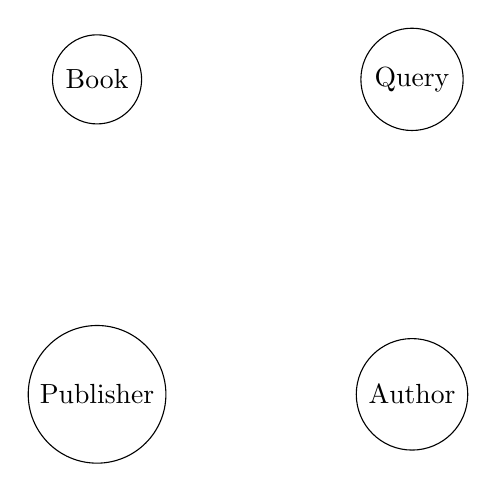
\begin{tikzpicture}
  \node[circle, draw] (n1) at (4,4) {Query};
  \node[circle, draw] (n2) at (0,4) {Book};
  \node[circle, draw] (n3) at (4,0) {Author};
  \node[circle, draw] (n4) at (0,0) {Publisher};
\end{tikzpicture}

In einer zweiten Iteration prüfen wir nun alle $fields$ Einträge des jeweiligen Types die vom Typ $OBJECT$ sind.
Beginnend im Query Type finden wir dort 3 Einträge in $fields$.
Jedes Feld besitzt einen Namen, in diesem Beispiel sind dies $book$, $author$ und $publisher$.

\begin{lstlisting}[language=json, caption={book Field},captionpos=b]
            {
              "name": "book",
              "description": null,
              "args": [
                {
                  "name": "id",
                  "description": null,
                  "type": {
                    "kind": "SCALAR",
                    "name": "ID",
                    "ofType": null
                  },
                  "defaultValue": null
                }
              ],
              "type": {
                "kind": "OBJECT",
                "name": "Book",
                "ofType": null
              },
              "isDeprecated": false,
              "deprecationReason": null
            }
\end{lstlisting}

\begin{lstlisting}[language=json, caption={author Field},captionpos=b]
            {
              "name": "author",
              "description": null,
              "args": [
                {
                  "name": "id",
                  "description": null,
                  "type": {
                    "kind": "SCALAR",
                    "name": "ID",
                    "ofType": null
                  },
                  "defaultValue": null
                }
              ],
              "type": {
                "kind": "OBJECT",
                "name": "Author",
                "ofType": null
              },
              "isDeprecated": false,
              "deprecationReason": null
            }
\end{lstlisting}

\begin{lstlisting}[language=json, caption={publisher Field},captionpos=b]
            {
              "name": "publisher",
              "description": null,
              "args": [
                {
                  "name": "id",
                  "description": null,
                  "type": {
                    "kind": "SCALAR",
                    "name": "ID",
                    "ofType": null
                  },
                  "defaultValue": null
                }
              ],
              "type": {
                "kind": "OBJECT",
                "name": "Publisher",
                "ofType": null
              },
              "isDeprecated": false,
              "deprecationReason": null
            }
\end{lstlisting}

Eine gerichtete Kante muss nun ausgehend vom Query-Knoten gezogen werden jeweils zum $type$ jedes einzelnen Feldes.
Die Kante erhält als Gewicht hierbei dann exakt die Feld-Definition.
So wird es später möglich aus Pfaden Querys zu bilden.
Nachdem alle Knoten iteriert wurden und die Felder untersucht sind, ergibt sich folgender Graph für unser Schema:

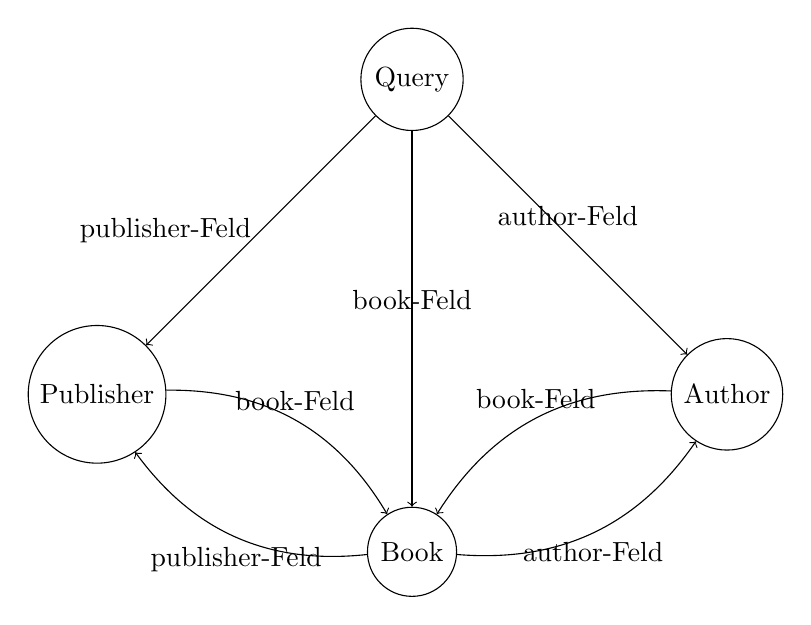
\begin{tikzpicture}
    \node[circle, draw] (n1) at (8,6) {Query};
    \node[circle, draw] (n2) at (8,0) {Book};
    \node[circle, draw] (n3) at (12,2) {Author};
    \node[circle, draw] (n4) at (4,2) {Publisher};

    \draw[->] (n1) -- node[above] {book-Feld} (n2);
    \draw[->] (n1) -- node[above] {author-Feld} (n3);
    \draw[->] (n1) -- node[left]  {publisher-Feld} (n4);
    \draw[->] (n2) to[bend right] node[below] {author-Feld} (n3);
    \draw[->] (n3) to[bend right] node[above] {book-Feld} (n2);
    \draw[->] (n2) to[bend left]  node[below] {publisher-Feld} (n4);
    \draw[->] (n4) to[bend left]  node[above] {book-Feld} (n2);
\end{tikzpicture}

Aus diesem Graphen können wir nun unsere Tests entwickeln.
Hierzu in den folgenden Kapiteln mehr.

\section{Pfade aus Graph bilden}

Dieser Schritt ist optional, je nach Implementation der Algorithmen für die Graphüberdeckung.
Es ist hierbei möglich einen generativen oder filternden Ansatz zu verfolgen.
Wird ein generativer Ansatz verfolgt, so wird direkt $6.3$ angewandt.
Alternativ generieren wir erstmal alle möglichen Simple-Paths (noch definieren - TODO) ausgehend von einem Startknoten.
Wir müssen die Simple-Paths vom Startknoten generierien, da in GraphQL nur Anfragen erlaubt sind, die in diesem Startknoten
beginnen.
Im allgemeinen Fall ist dies der Knoten $Query$
Diese Simple-Paths werden dann im nächsten Schritt gefiltert durch das jeweilige Coverage-Kriterium.
In unserem Beispielgraphen sind die Simple-Paths folgende:

\begin{itemize}
    \item (Query, Book)
    \item (Query, Author)
    \item (Query, Publisher)
    \item (Query, Author, Book)
    \item (Query, Publisher, Book)
    \item (Query, Book, Author)
    \item (Query, Book, Publisher)
    \item (Query, Publisher, Book, Author)
    \item (Query, Author, Book, Publisher)
\end{itemize}

\section{Coverage-Pfade ermitteln}

Wie zuvor unterschieden, gibt es zwei Verfahren um die Pfade zu generieren.
Wir werden hier beide Verfahren getrennt voneinander
Zuerst betrachten wir den filternden Ansatz da er thematisch zum vorherigen Kapitel abschließend ist.

\subsection{filternder Ansatz}
Aus der zuvor gewonnen Menge an Simple-Paths können wir nun je nach Coverage-Kriterium die Pfade, die für unser Coverage-Kriterium
wichtig sind, herausfiltern.
Exemplarisch nutzen wir hierfür einmal die Prime-Path Coverage.
Es ist jedoch denkbar auch andere Coverage-Kriterien zu verwenden.
Wir erinnern uns: Ein Prime-Path ist ein Pfad, der weder selbst Teil eines anderen Pfades ist noch sich wiederholt.
Dies bedeutet, dass wir alle Pfade aus den Simple-Paths danach filtern müssen, dass diese weder Teilpfad eines anderen Pfades sind
noch, dass sie sich wiederholen.
Hier kann man folgenden Pseudo-Code nutzen um einen Filter für PrimePaths zu entwickeln:

\begin{verbatim}
    Input: alle_Pfade

    prime_paths = []

    Für alle_Pfade:
        Wenn istPrimePfad(Pfad, alle_Pfade):
            prime-paths =+ Pfad
        Sonst verwerfe Pfad

    return prime_paths


    Funktion istPrimePfad(möglicherPrimePath, alle_Pfade):
        Für pfad in alle_Pfade:
            Wenn möglicherPrimePath != pfad and istTeilpfad(möglicherPrimePath, pfad)
                return False
        return True

    Funktion istTeilpfad(möglicherPrimePath, pfad):
        Wenn Länge(möglicherPrimePath) > Länge(pfad):
            return False
        Für jeden TeilPfad von Pfad:
            Wenn TeilPfad = möglicherPrimePath:
                return True
        return False

\end{verbatim}

Dieser PseudoCode bewirkt, dass wir für jeden Pfad ermitteln ob dieser ein PrimePath ist.
Hierbei iterieren wir über jeden einzelnen Pfad und prüfen ob dieser ein PrimePfad ist.
Hierbei fügen wir einen Pfad der Liste alle Prime-Paths hinzu, wenn dieser die Funktion istPrimePfad mit $True$ erfüllt.
Die Funktion liefert hierbei nur $True$ zurück, wenn der Pfad sich nicht wiederholt und er die Funktion istTeilpfad mit False belegt.
Somit erreichen wir genau, dass nur diejenigen Pfade mit $True$ in die Liste gegeben werden, die genau unsere eingangs definierten Bedinungen
erfüllen.
Nutzen wir nun diesen Pseudo-Code auf unserer Menge der SimplePaths so bekommen wir folgende PrimePaths:

\begin{itemize}
    \item (Query, Book, Author)
    \item (Query, Publisher, Book, Author)
    \item (Query, Book, Publisher)
    \item (Query, Author, Book, Publisher)
\end{itemize}

Diese filternde Methode ist im Allgemein einfacher zu implementieren, bietet jedoch einen großen Nachteil:
Die Generierung der SimplePaths ist sehr rechenintensiv und außerdem werden hierfür Pfade nur entfernt aus der größeren Menge.
Dies bedeutet, dass die SimplePaths eine schon sehr gute Abdeckung bieten und die PrimePaths den Testraum nur potentiell verkleinern da wir eben
nur aus der SimplePath Menge dann Pfade löschen.
Die Methode des Filterns eignet sich also am ehesten für kleine Schemas da hier das bilden der SimplePaths noch relativ rechenarm
ist und zur Validierung von verschiedenen CoverageKriterien da die generative Implementierung komplexer ist.
Hierdurch kann man also vorher überprüfen, ob es sich lohnt ein anderes CoverageKriterium mittels generativem Ansatz zu implementieren.
Der generative Ansatz gewinnt dann an Bedeutung wenn die GraphQL-Schemas größer werden da so Rechenzeit gespart werden kann.
Es sei außerdem erwähnt, dass die Ausführungszeit der Tests auch relevant sein kann und somit die Anzahl an Pfaden durch Filtern reduziert werden muss.

\subsection{generativer Ansatz}

Mittels eines generativen Ansatzes lassen sich von einem gegebenen Startpunkt die Pfade ermitteln, welche die gewünschte Coverage
erreichen.
Hierbei unterscheidet sich der konkrete Ansatz je nach Coverage-Kriterium wieder.
Im allgemeinen wird eine Funktion $generatePaths(Startpunkt, Graph)$ erwartet.
Wobei der Startpunk im Allgemeinen der $Query$ Knoten ist und $Graph$ den kompletten Graphen abbildet.
Erwarteter Rückgabewert der Methode ist eine Liste von Pfaden die das jeweilige CoverageKriterium erfüllen.
Wir werden auch hier wieder einen Pseudo Code vorstellen, der für die Generierung von Prime-Paths zuständig ist aber allerdings
den generativen Ansatz verfolgt.

\begin{verbatim}

    testPfade = []
    Generiere_Prime_Pfade(startknoten, [], testPfade, Graph)


    Function Generiere_Prime_Pfade(Knoten, Pfad, testPfade, Graph):
        Füge den Knoten dem Pfad hinzu
        Für alle FolgeKnoten von Knoten:
            Wenn FolgeKnoten nicht in Pfad:
                generiere_Prime_Pfade(FolgeKnoten, testPfade, Pfadliste, Graph)
        Wenn Ist_PrimePfad?(Pfad, testPfade):
            Füge Pfad den testPfaden hinzu

    Function Ist_PrimePfad?(neuerPfad, testPfade):
        Für alle Pfade in TestPfade:
            Wenn neuerPfad ein Teilpfad eines Pfades ist
                return False
        return True

\end{verbatim}

Der Pseudocode startet im Startpunkt des Graphens und iterriert dann rekursiv über die Folgeknoten des Graphens.
Hierbei wird stets in Beachtung gehalten, dass ein Knoten in einem Pfad nicht zweimal vorkommen kann.
So vermeiden wir Kreise und eine mögliche, unendlichen Generierungsraum.
Für jeden generierten Pfad wird dann überprüft ob dieser ein Prime-Path ist.
Dies ist der Fall wenn er kein Teilpfad eines anderen Pfades ist und sich nicht selbst wiederholt.
Wir stellen sicher, dass der Pfad sich nicht wiederholen kann indem wir Kreise erst gar nicht zulassen.
Im zweiten Schritt prüfen wir dann ob ein Pfad ein Teilpfad ist.
Endergebniss sind dann die Prime-Paths des Graphens.
Dieser Code ergibt dann folgende Pfade für die PrimePath-Coverage die den Graphen überdecken:

\begin{itemize}
    \item (Query, Book, Author)
    \item (Query, Publisher, Book, Author)
    \item (Query, Book, Publisher)
    \item (Query, Author, Book, Publisher)
\end{itemize}

Wir sehen diese sind identisch zum filternden Ansatz.

\section{Query aus Pfad ermitteln}

Da wir nun die Pfade, je nach Coveragekriterium ermittelt haben müssen wir nun eine Query aus diesen Pfaden bilden.
Hierbei nutzen wir diverse Hinweise die im GraphQL-Schema gegeben werden und einen Teil der Arbeit aus \cite[Property-Based Testing]{property-based-testing}.
Jeder ermittelte Pfad startet im Query-Knoten.
Da wir zuvor den Kanten jeweils die Feldattribute mitgegeben haben, können wir nun sehr einfach ermitteln welche
Operationen wir ausführen müssen, um von einem Knoten zum nächsten zu kommen.
Dies bedeutet, dass die Kanteninformationen ausreichen, um eine Query zu bilden.
Wir gehen hierbei den kompletten Pfad ab und geben einen Query-String zurück der für GraphQL zulässig ist.
Eine valide GraphQL-Query beginnt mit $\{ \}$ und folgt dann mit der ersten Felddefinition.
Eine Felddefinition kann vom Type $SCALAR$ oder $OBJECT$ sein.
Ist ein Feld vom Type $SCALAR$ so kann dieses einfach der Query hinzugefügt werden als erwartetes Feld.
GraphQLs Spezialität ist es, dass nur wirklich angeforderte Felder in einer Response existieren.
Im Kontext des Integrationstesten wollen wir aber alle möglichen Felder abfragen einfach um sicher zu gehen, dass
diese korrekt Installiert wurden.
Es wäre denkbar auch Variationen der einzelnen Felder zu implementieren, dass nicht in jeder Query immer alle Felder
eines Typen berücksichtig werden, dies wird hier jedoch zuerst vernachlässigt und wir inkludieren alle Felder.
Ist ein Feld vom Type $OBJECT$ so bedeutet dies, dass dieses Feld nur angegeben werden muss, wenn der nachfolgende Knoten im Pfad
exakt den Typen dieses Feldes hat!
Das Feld wird dann wieder eingeleitet durch $\{ \}$.
Innerhalb dieser Felder ist nun wieder jedes Feld des Typen $SCALAR$ hinzuzufügen und das Feld des nächsten Knotens zu suchen sowie hinzuzufügen.
Sollte ein Feld vom Type $OBJECT$ Argumente benötigen, so steht dies im Schema und wir können diese generieren.
Input-Argumente können vom Type $INPUT-OBJECT$ sein oder $SCALAR$.
Sollte es ein Scalar Type sein, so bedienen wir uns der Methode aus \cite[Property-based Testing]{property-based-testing} und generieren
jeweils Zufallsargumente in Form des jeweiligen Datentyps.
Ein String bedeutet also, dass wir einen beliebig langen String erzeugen, ein Integer ist eine Zufallszahl usw.
Sollte das Argument vom Type $INPUT-OBJECT$ sein so lässt es sich in seine Bestandteile zerlegen welche auch wieder $SCALAR$ Types sind und
dann werden diese auch zufällig entsprechend generiert und dem $INPUT-OBJECT$ Type entsprechend angeordnet.
Argumente folgen dann jeweils zwischen dem Namen des Felds vom $OBJECT$ und den sich öffnenden, geschweiften Klammern.
Für unser Beispiel von vorher bedeutet dies also, dass wenn wir aus dem Pfad $(Query, Book, Publisher)$ eine Query bilden wollen, wir folgende
Schritte zu erfüllen haben:

\begin{enumerate}
    \item Finde Kante von $Query$ zu $Book$
    \item Ermittel ob die Kante $(Query, Book)$ Argumente benötigt.
    \item Ermittel alle $SCALAR$ Types die $Book$ definiert.
    \item Ermittel die Kante von $Book$ zu $Publisher$
    \item Ermittel ob die Kante $(Book, Publisher)$ Argumente benötigt.
    \item Ermittel alle $SCALAR$ Types die $Publisher$ definiert. (Pfad zuende daher kein Folge-Typ)
    \item Baue Query-String aus den erlangten Informationen
\end{enumerate}

Wir werden nun Schritt für Schritt alle Schritte einzeln durchgehen und eine Query generieren.

\begin{figure}[htbp]
    \centering
    \begin{minipage}[t]{0.5\textwidth}
        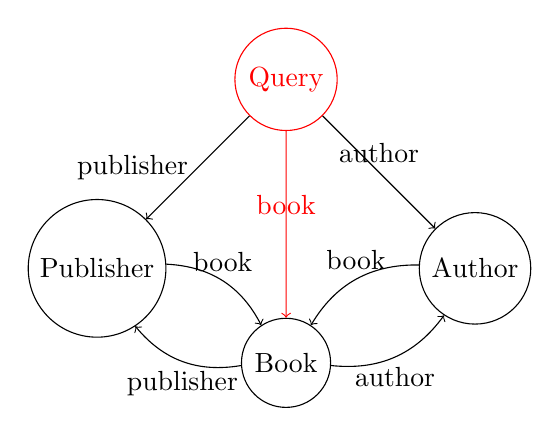
\begin{tikzpicture}[scale=0.6, baseline=(current bounding box.north)]
        \node[circle, draw, red] (n1) at (8,6) {Query};
        \node[circle, draw] (n2) at (8,0) {Book};
        \node[circle, draw] (n3) at (12,2) {Author};
        \node[circle, draw] (n4) at (4,2) {Publisher};

        \draw[->, red] (n1) -- node[above] {book} (n2);
        \draw[->] (n1) -- node[above] {author} (n3);
        \draw[->] (n1) -- node[left]  {publisher} (n4);
        \draw[->] (n2) to[bend right] node[below] {author} (n3);
        \draw[->] (n3) to[bend right] node[above] {book} (n2);
        \draw[->] (n2) to[bend left]  node[below] {publisher} (n4);
        \draw[->] (n4) to[bend left]  node[above] {book} (n2);
        \end{tikzpicture}
    \end{minipage}%
    \begin{minipage}[t]{0.5\textwidth}
        Wir betrachten die Kante (Query, Book).
        Durch unsere vorherige Definition des Graphens wissen wir, dass diese Kante das Attribut $book$ trägt und uns somit hinweist, welches Feld wir benötigen
        um diese Kante in unserer Query abzubilden.
        Dieses entspricht $Listing 6.6$ und wir erkennen, dass das Book-Field ein Argument $id$ vom Typ $ID$ besitzt.
        Daher wissen wir, dass wir dem Book-Feld ein Argument $(id: RandomString)$ mitgeben müssen.
        Im nächsten Schritt suchen wir noch alle $SCALAR$ Types die in Book definiert sind.
        Hierzu schauen wir in der \hyperref[Schema-Response]{minimal-schema-response} im Type $Book$ nach und finden,
        dass ein $Book$ die Felder $title$ und $id$ vom $SCALAR$ Type hat.
    \end{minipage}
\caption{Schritte 1 - 3}
\end{figure}

\begin{figure}[htbp]
    \centering
    \begin{minipage}[t]{0.5\textwidth}
        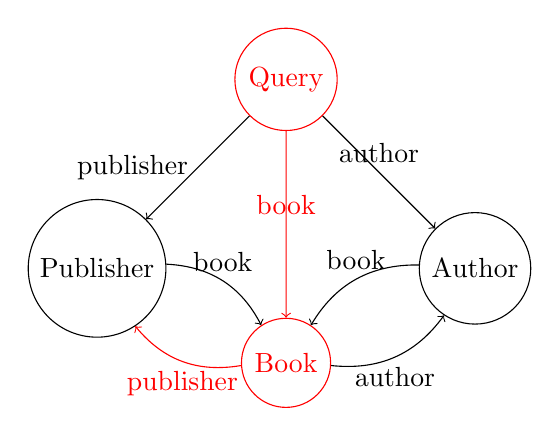
\begin{tikzpicture}[scale=0.6, baseline=(current bounding box.north)]
        \node[circle, draw, red] (n1) at (8,6) {Query};
        \node[circle, draw, red] (n2) at (8,0) {Book};
        \node[circle, draw] (n3) at (12,2) {Author};
        \node[circle, draw] (n4) at (4,2) {Publisher};

        \draw[->, red] (n1) -- node[above] {book} (n2);
        \draw[->] (n1) -- node[above] {author} (n3);
        \draw[->] (n1) -- node[left]  {publisher} (n4);
        \draw[->] (n2) to[bend right] node[below] {author} (n3);
        \draw[->] (n3) to[bend right] node[above] {book} (n2);
        \draw[->, red] (n2) to[bend left]  node[below] {publisher} (n4);
        \draw[->] (n4) to[bend left]  node[above] {book} (n2);
        \end{tikzpicture}
    \end{minipage}%
    \begin{minipage}[t]{0.5\textwidth}
        Im Folgenden wollen wir die Kante (Book, Publisher) betrachten um unseren Pfad abzuschließen.
        Wie zuvor finden wir, dass die Kante das Attribut $publisher$ trägt.
        Wir müssen nun allerdings nicht im Query-Type das Feld $publisher$ suchen sondern im aktuell befindlichen Knoten (Book).
        Hierbei finden wir, dass vom Type $Book$ das Feld $publisher$ kein Argument benötigt.
        Wir müssen daher nur noch ermitteln, welche Felder vom $SCALAR$ Type in Publisher definiert werden.
        Dies sind die Felder $id$ und $name$.
    \end{minipage}
    \caption{Schritte 4 - 6}
\end{figure}

\begin{figure}[htbp]

    \begin{center}
        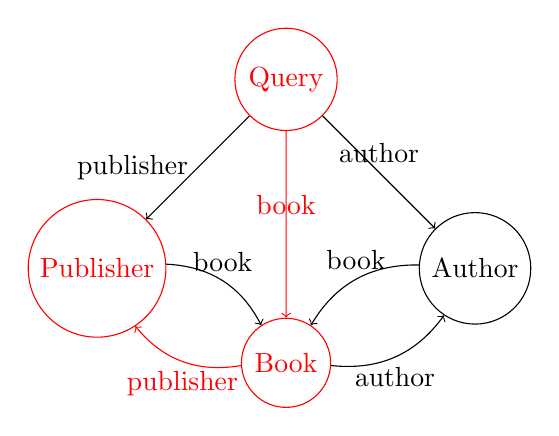
\begin{tikzpicture}[scale=0.6, baseline=(current bounding box.north)]
        \node[circle, draw, red] (n1) at (8,6) {Query};
        \node[circle, draw, red] (n2) at (8,0) {Book};
        \node[circle, draw] (n3) at (12,2) {Author};
        \node[circle, draw, red] (n4) at (4,2) {Publisher};

        \draw[->, red] (n1) -- node[above] {book} (n2);
        \draw[->] (n1) -- node[above] {author} (n3);
        \draw[->] (n1) -- node[left]  {publisher} (n4);
        \draw[->] (n2) to[bend right] node[below] {author} (n3);
        \draw[->] (n3) to[bend right] node[above] {book} (n2);
        \draw[->, red] (n2) to[bend left]  node[below] {publisher} (n4);
        \draw[->] (n4) to[bend left]  node[above] {book} (n2);
        \end{tikzpicture}
    \end{center}
    Wir haben nun unseren Pfad vollständig abgebildet.
    Nun müssen wir aus den gewonnenen Informationen einen Query-String bilden.
    Hierfür starten wir mit zwei geschweiften Klammern:
    \begin{lstlisting}[language=GraphQL]
        {
        }
    \end{lstlisting}


    Als Erstes fügen wir das gewählte Feld "Book" mit seinem Argument hinzu und fügen wieder zwei geschweifte Klammern hinzu für die Felder des Types.
    In diese geschweiften Klammern kommen zuerst die $SCALAR$ Types.
    Dadurch erhalten wir die Query:

    \begin{lstlisting}[language=GraphQL]
        {
            book(id: RandomString){
                id
                title
            }
        }
    \end{lstlisting}

    Danach folgt das Feld, das die nächste Kante abbildet.
    In diesem Fall hat es kein Argument, aber wir fügen geschweifte Klammern mit dem Kantenbezeichner hinzu.
    Dadurch erhalten wir die Query:

    \begin{lstlisting}[language=GraphQL]
        {
            book(id: RandomString){
                id
                title
                publisher {}
            }
        }
    \end{lstlisting}


    Zum Schluss fügen wir alle $SCALAR$-Felder des $Publisher$-Typs hinzu, um auch die letzte Kante abzubilden.
    Diese Felder sind $id$ und $name$.
    Die fertige Query lautet also:

    \begin{lstlisting}[language=GraphQL]
        {
            book(id: RandomString){
                id
                title
                publisher {
                    id
                    name
                }
            }
        }
    \end{lstlisting}

    Diese Query deckt unseren Pfad $(Query, Book, Publisher)$ ab.
    \caption{Schritt 7}
\end{figure}

Dieses Prozedere muss nun mit allen ermittelten Pfaden durchgeführt werden um aus den Pfaden die Querys zu generieren welche
die Tests darstellen.
Da wir uns bei der Generierung der Argumente für Querys auf~\cite[Property-based Testing]{property-based-testing} beziehen ist es
unter Umständen möglich, dass Querys Argumente bekommen, die nicht zur zugrundeliegenden Datenstruktur passen.
D.h. in der Standardmethode wird für ein zufälligen Integer-Wert direkt der gesamte Integer Wertebereich genutzt.
Ist der Datenraum jedoch sehr klein, so kann es sein, dass kein einziger exisitenter Wert getroffen wird und die
Query nur eine leere Antwort wiedergibt da das Element nicht gefunden wurde.
Hier kommt es auf die spezielle Implementierung einerseits des SUT an andererseits auch auf die Programmierung der
Argumentgeneratoren.
Hierzu jedoch im Praxisteil mehr.

\section{Test ausführen \& Testauswertung}

Für die Testausführung halten wir uns wieder ähnlich zum \cite[Property-based Testing]{property-based-testing}.
Durch die zufällige Argument-Generierung ist es leider nicht möglich, strukturiert zu überprüfen, ob die zurückgelieferten Daten
passend sind zu dem was wir angefragt haben.
Hier hat unser Ansatz die selben Probleme wie das \cite[Property-based Testing]{property-based-testing}.
Zur Überprüfung der Querys stellen wir diese ganz einfach per HTTP-Post an den zu testenden GraphQL-API Endpunkt.
In der Response erhalten wir dann einen StatusCode welcher üblicherweise zwischen 2XX und 5XX liegt.
Wir werden nun die einzelnen StatusCodes aufbrechen, da diese inherent wichtig sind für unsere Testauswertung.
Responses von 2XX werden in Kapitel $Positive Tests$ behandelt, 4XX in Falsch-Negative Tests und 5XX in Negative Tests.

\subsection{Positive Tests}
Einen positiven Test zeichnet aus, dass dieser einen HTTP-Response Code von 2XX erhält.
Im Allgemeinen Fall sagt dies aus, dass alles mit der Anfrage gut lief und wir eine Antwort erhalten haben die
unseren Erwartungen entspricht.
Dies bedeutet, dass für unser Beispiel zuvor die Query
\begin{lstlisting}[language=GraphQL]
        {
            book(id: RandomString){
                id
                title
                publisher {
                    id
                    name
                }
            }
        }
\end{lstlisting}

eine Response zurückgeliefert hat die dieser erwarteten Struktur entspricht.
Im Allgemeinen wird also erwartet, dass unsere Query dann zum Beispiel diese Response liefert:

\begin{lstlisting}[language=GraphQL]
        {
            "data": {
                "book": {
                    id: "1",
                    title: "Moby Dick"
                    publisher: {
                        id: "1",
                        name: "Testverlag"
                    }
                }
            }
        }
\end{lstlisting}

Allerdings bedeutet dies, dass wir den glücklichen Fall haben, dass das Argument von $book(id: Argument)$ die passende
ID für ein Buch war.
Dadurch, dass wir jedoch unsere Eingabevariabeln zufällig generieren, können wir nicht davon ausgehen, dass uns dies regelmäßig gelingt.
Sehr wahrscheinlich wird eine Response zwar den Status-Code 200 liefern allerdings werden die enthaltenen Daten der Response
dieses Format haben:

\begin{lstlisting}[language=GraphQL, caption={mangelhafte Response}]
        {
            "data": {
                "book": null
            }
        }
\end{lstlisting}


Gegen dieses Verhalten wollen wir Maßnahmen einführen damit sichergestellt werden kann, dass zumindest eine signifikante Aussage über die
tatsächliche Testabdeckung ausgeführt werden kann - denn wie zuvor erwähnt, werden Funktionen tiefer im Pfad erst ausgeführt, wenn das Objekt zuvor
erfolgreich ermittelt wurde.

\subsubsection{Unterschiede in den Pfadlängen}
Diese Methode verbessert zwar nicht die Testergebnisse allerdings gibt Sie uns Informationen darüber wie viel von unserem Pfad in Wirklichkeit
abgedeckt wurden.
Dadurch lässt sich der Erfolg der Tests besser abschätzen da wir so messen können ob die Querys wirklich die Funktionen ausgeführt haben.
Hierzu wird die Pfadlänge des Pfades der zur Erstellung der Query genutzt wurde als erwartete Pfadlänge angenommen.
Die Pfadlänge der Antwort wird dann als tatsächliche Pfadlänge genommen.
Der Unterschied zwischen erwarteter und tatsächlicher Pfadlänge ist dann unser Auswertungsmerkmale für diesen speziellen Test.
Die Pfadlänge der Response ist die maximale Tiefe der JSON-Response verringert um 1.

\[ \text{Tiefe des Pfades} = \text{Tiefe des JSON-Response-Objekts} - 1 \]

Demnach hätte folgende Response eine Tiefe von 2
\begin{lstlisting}[language=GraphQL, caption={vollständige Response}]
    {
        "data": {
            "book": {
                id: "1",
                title: "Moby Dick"
                publisher: {
                    id: "1",
                    name: "Testverlag"
                }
            }
        }
    }
\end{lstlisting}

Und die leere Antwort hätte eine Tiefe von 1

\begin{lstlisting}[language=GraphQL, caption={mangelhafte Response}]
    {
        "data": {
            "book": null
        }
    }
\end{lstlisting}

Der Unterschied zwischen beiden signalisiert uns dann, ob die erfolgreiche Query denn die komplette Query durchlaufen ist oder nur ein Teil
davon.
Hierdurch gelingt uns eine Auswertung.
Wir können die Pfadlängen aller erwarteten Pfade addieren, das gleiche können wir auch mit den tatsächlichen Pfaden machen.
So erreichen wir zwei Zahlen und mit diesen können wir eine Prozentuale Einschätzung abgeben, wieviel Prozent unserer Tests
insgesamt ausgeführt wurden.
Wir rechnen hierfür:

\[ \text{Prozent der tatsächlichen Abdeckung} = \frac{\text{tatsächliche Gesamtpfadlänge}}{\text{erwartete Gesamtpfadlänge}} * 100 \]

Wir sollten einen Wert nahe der 100\% anstreben.
Dies würde bedeuten, dass unsere generierten Tests auch alle Funktionen getestet haben.
Andernfalls bedeutet ein Prozentsatz unter 100\% eben, dass nicht alle Funktionen tatsächlich von den Querys überdeckt wurden.


\subsubsection{Zufallsgeneratoren der Argumente}

Unser zuvor vorgestellte Methode liefert uns einen Hinweis darauf, wie gut unsere Querys tatsächlich geteste haben.
Dieser Ansatz verfolgt das Ziel die Querys eine bessere tatsächliche Abdeckung zu erreichen.
Hierbei ist das Anpassen der Generatoren für die Argumente im Fokus.
In der vorgestellten Methode unter $6.4$ erstellen wir komplett zufällig Argumente für die Funktionen.
Dies bedeutet, dass z.B. der Type $ID$ als String gewertet wird.
Dieser Type ist meist sehr bedeutend, da dieser häufig als Argument angegeben wird und eine spezielle Struktur hat.
Es hängt natürlich stark von der eigenen Implementierung der GraphQL-API ab allerdings wenn in der Implementierung
eine $ID$ definiert ist als Zahlenstring, so kann es sich durchaus lohnen, dass der Argumentgenerator für die ID auch speziell
auf Zahlenstrings angepasst wird.
Alternativ kann auch eine Liste aller existenten IDs angegeben werden und zufällig ausgewählt werden.
Wir erhöhen hierdurch letztendlich einfach die Chance, dass zufällig eine tatsächliche ID gewählt wird die auch
in den Daten des SUT existent ist.
Eine exakte Vorgehensweise für diese Methode ist allerdings stark abhängig vom System das zu testen ist und daher stark Fall abhängig.

\subsubsection{Anzahl der Querys}

Wir haben bisher eingeführt, dass wir messen können, welche Abdeckung unsere Querys tatsächlich haben und haben festgelegt wie wir diese Verbessern können.
Da wir zufallsbasiert die Argumente generieren können wir nicht davon ausgehend, dass die erste Query direkt passt und eine ideale Pfadlänge bietet.
Es kann passieren, muss aber nicht.
Erhöhen wir jetzt die Anzahl der generierten Querys pro Pfad, so erhöhen wir auch die Wahrscheinlichkeit,
dass zumindest eine Query die ideale Pfadlänge für diesen Pfad erreicht.
Hierfür müssen wir $Schritt 7.$ aus $6.4$ so oft wie gewünscht wiederholen, sodass wir verschiedene Querys mit verschiedenen Argumenten erhalten.
Bei dieser Methode ist nämlich wichtig, dass sich die Argumente der Querys verändern da wir sonst einfach mehrfach die selbe Query stellen mit der
gleichen zu erwartenden Antwort.

\subsection{Falsch-Negative Tests}

Responses mit dem HTTP-StatusCode 4XX sind zu sehr hoher Wahrscheinlichkeit Fehler in der Query.
Fehler in der Query können passieren wenn falsche Argument-Typen angegeben werden, ein Syntaxfehler auftritt oder
zwingende Argumente fehlen.
Eine konkrete Implementierung sollte beachten, dass diese Fehler vorkommen können und sie explizit als Falsch-Negativen Tests werten dann
hierbei hat das SUT nichts falsch gemacht sondern die Implementierung des Testtools ist falsch.
Einige GraphQL-APIs reagieren mit einem 400er Fehlercode auf nicht gefundene Einträge.
Dies ist jedoch abhängig vom SUT und muss gesondert betrachtet werden.

\subsection{Negative Tests}

Sollte eine Response den StatusCode 5XX erhalten, so haben wir einen tatsächlichen Fehler in der Programmierung gefunden
da der Statuscode auf einen Internen ServerFehler hinweist.
Ein Internet Serverfehler entspricht einer falschen Programmierung also einem Fehler den unsere Methode gefunden hat.
Typischerweise liefert eine GraphQL-API den exakten Fehler mit.
Aus dieser Fehlermeldung kann dann der Entwickler Schlüsse ziehen wieso dieser Fehler auftrat.
Sollte eine GraphQL-API diesem Testsystem standhalten und keine Response mit 500er zurückliefern, so bedeutet dies nicht,
dass die GraphQL-API keinen Fehler enthält.
Man kann also nicht davon ausgehen, dass diese Methode alle Fehler findet die in einer GraphQL-API existieren.
Dies liegt einerseits daran, dass nicht jede Kante getestet wird.
Andererseits auch daran, dass die Response nicht überprüft wird auf ihre tatsächlichen zurückgegebenen Daten.
So ist es denkbar, dass Tests zwar positiv sind da sie Daten mit StatusCode 200 zurückliefern, diese allerdings
nicht den erwarteten Daten entsprechen.
Hierzu sollen alle generierten Tests sowie ihre Response abgespeichert werden damit diese von einem Entwickler manuell
noch untersucht werden können.

\section{Zusammenfassung der Methode und struktureller Vergleich mit Property-based Testing}

Wir wollen im folgenden die eben vorgestellte Methode noch einmal kurz zusammenfassen damit diese übersichtlicher wird.
Unsere hier vorgestellte Methode funktioniert grob gesehen so:

\begin{center}
    \includegraphics[width=\textwidth,height=\textheight,keepaspectratio]{img/methode}
\end{center}

Wie zu sehen, ist der ganz grobe Ablauf ähnlich zum \cite[Property-based Testing]{property-based-testing} allerdings unterscheidet sich die
Methode in einigen Teilen sehr stark vom \cite[Property-based Testing]{property-based-testing}.
Wir fügen in unserer Methode den Schritt hinzu, dass wir einen Graphen erstellen welcher die Knoten und Kanten des GraphQL-Schemas repräsentiert
während in \cite[Property-based Testing]{property-based-testing} ausgehend vom Query-Type zufällig bis zu einer bestimmten Pfadlänge (dem Rekursionslimit)
die Pfade gebildet werden indem immer zufällig Felder hinzugefügt werden.
Durch unsere Methode erreichen wir, dass Pfade jeder Länge, die durchaus länger sein können als ein definiertes Rekursionslimit, abgedeckt werden und
somit die Tests eine bessere Coverage erreichen können.
Unser Ansatz erlaubt es außerdem, verschiedene Coverage-Kriterien zu implementieren.
So ist man nicht gezwungen auf einer Methode zu verharren sondern kann je nach Implementierung die Pfadgenerierung anpassen nach den individuellen
Anforderungen ohne, dass in anderen Schritten etwas geändert werden muss.
Bei der Umwandlung der Pfade in Querys unterscheidet sich unser Ansatz ein wenig von \cite[Property-based Testing]{property-based-testing}.
In unserer Methode generieren wir aus dem Pfad direkt die Query und generieren die nötigen Argumente ''on-the-fly'' während sie erkannt werden.
Im Property-based Ansatz wird ein Datenobjekt als ganzes erstellt, dass die Query später generieren kann.
In der technischen Umsetzung unterscheiden sich beide Methoden, im Ergebnis bekommen Sie jedoch strukturell gleiche Querys.
Die Ausführung der Tests hingegen unterscheidet sich überhaupt nicht mehr zum \cite[Property-based Testing]{property-based-testing}.
Einzig und allein unsere Einführung der erwarteten vs. tatsächlichen Pfadlänge ist ein neuer Ansatz der die Qualität der zu testenden Querys
messbar macht - dies fehlt im \cite[Property-based Testing]{property-based-testing}.
Dort ist man im unklaren darüber wie gut die Tests genau getestet haben und ob die erwartete Coverage auch mit der tatsächlichen Übereinstimmt.
\\
\\
Wir haben nun unsere Methode im groben vorgestellt und Unterschiede zum schon bestehenden Ansatz \cite[Property-based Testing]{property-based-testing} erörtert.
Im folgenden wollen wir uns der praktischen Umsetzung dieser Methode widmen und einen Prototypen entwickeln.
Dieser Prototyp soll dann gegen das \cite[Property-based Testing Tool]{property-based-testing} antreten und möglichst zeigen, dass die eben entwickelte Methode
eine Verbesserung darstellt.






